\documentclass[12pt]{article}

\usepackage{setspace}
\usepackage{caption}
\usepackage{subcaption}
\usepackage{float}
\usepackage{makecell}
\usepackage{amsmath}
\usepackage{graphicx}
\usepackage{subfig}
\graphicspath{ {./images/} }
\usepackage[utf8]{inputenc}
\usepackage[russian]{babel}
\usepackage{geometry}
 \geometry{
 a4paper,
 left=20mm,
 right=20mm,
 top=20mm,
 bot=20mm,
 }

\begin{document}

\begin{titlepage}
\begin{center}
    НАЦИОНАЛЬНЫЙ ИССЛЕДОВАТЕЛЬСКИЙ УНИВЕРСИТЕТ ИТМО \\
    Факультет систем управления и робототехники \\
    \vspace*{10\baselineskip}
    {\LARGEЭлектротехника} \\
    \ \\
    \ \\
    \begin{spacing}{1.5}
    {\large Лабораторная работа №23 \\
    СИНТЕЗ СЧЕТЧИКА С ПРОИЗВОЛЬНЫМ МОДУЛЯ СЧЕТА $M < 2^n$ \\
    \ \\
    Вариант 3R382}
    \end{spacing} \\
    \ \\
    \vspace*{10\baselineskip}
    \hfill {Студент: Кирбаба Д.Д.\ \ \ \ \ \ \ \ \ } \\
    \hfill {Группа: R3338\ \ \ \ \ \ \ \ \ \ \ \ \ \ \ \ \ \ \ \ \ } \\
    \hfill {Преподаватель: Китаев Ю.В.} \\
    \mbox{}
    \vfill {г. Санкт-Петербург\\2023}
\end{center}
\end{titlepage}

\subsection*{Цель работы}
Изучение построения и функционирования счетчиков.

\subsection*{Ход работы}

Начальные данные:
\[
    M = 9, \ D \rightarrow JK \rightarrow JK \rightarrow D.
\]

Число триггеров равно 4. \\

\begin{figure}[H]
    \centering
    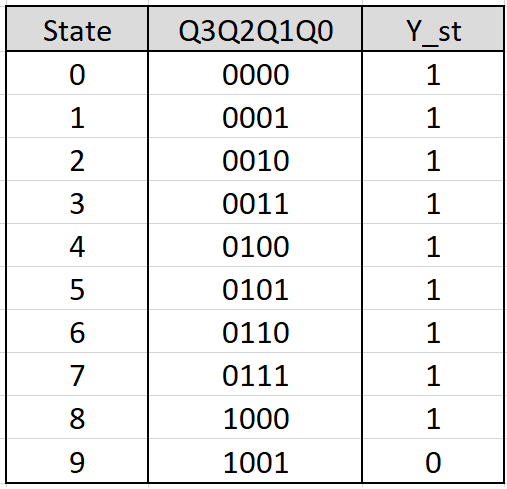
\includegraphics[width=0.5\textwidth]{states.png}
    \caption{Таблица состояний.}
    \label{fig:states}
\end{figure}

Вычислим алгебраическое выражение для $Y_{st}$ с помощью таблицы Карно:
\begin{figure}[H]
    \centering
    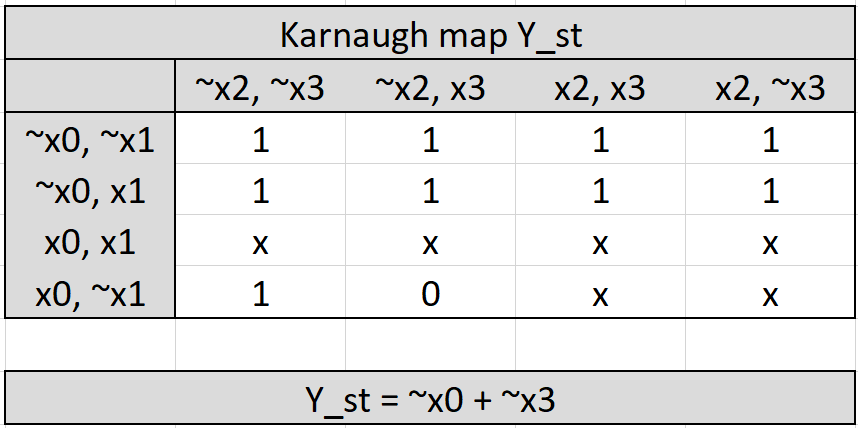
\includegraphics[width=0.7\textwidth]{kar.png}
    \caption{Таблица Карно и выражение для функции.}
    \label{fig:kar}
\end{figure}

Сконструированная блок-схема для реализации счетчика:
\begin{figure}[H]
    \centering
    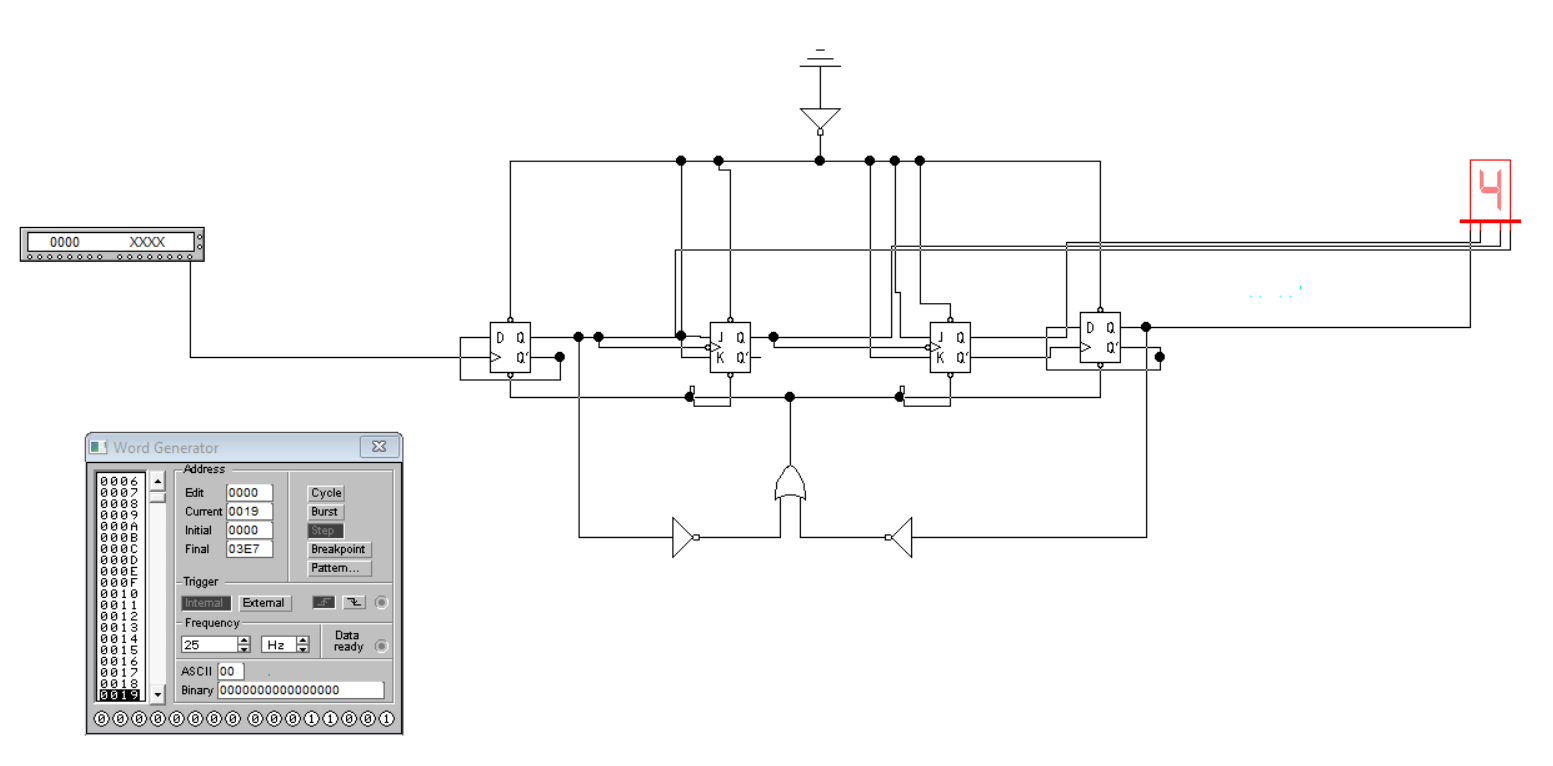
\includegraphics[width=\textwidth]{scheme.png}
    \caption{Блок-схема счетчика с обратной связью.}
    \label{fig:scheme}
\end{figure}

При контроле состояний, видно, что счетчик выполняет поставленную задачу, а именно индикатор последовательно показывает числа $0, \ 1, \ 2, \ 3, \ 4, \ 5, \ 6, \ 7, \ 8$ и затем сбрасывает состояния и цикл начинается заново. \\
\ \\
Теперь отключим обратную связь и снимем код с обратных выходом, тем самым переделав счетчик в вычитающий:
\begin{figure}[H]
    \centering
    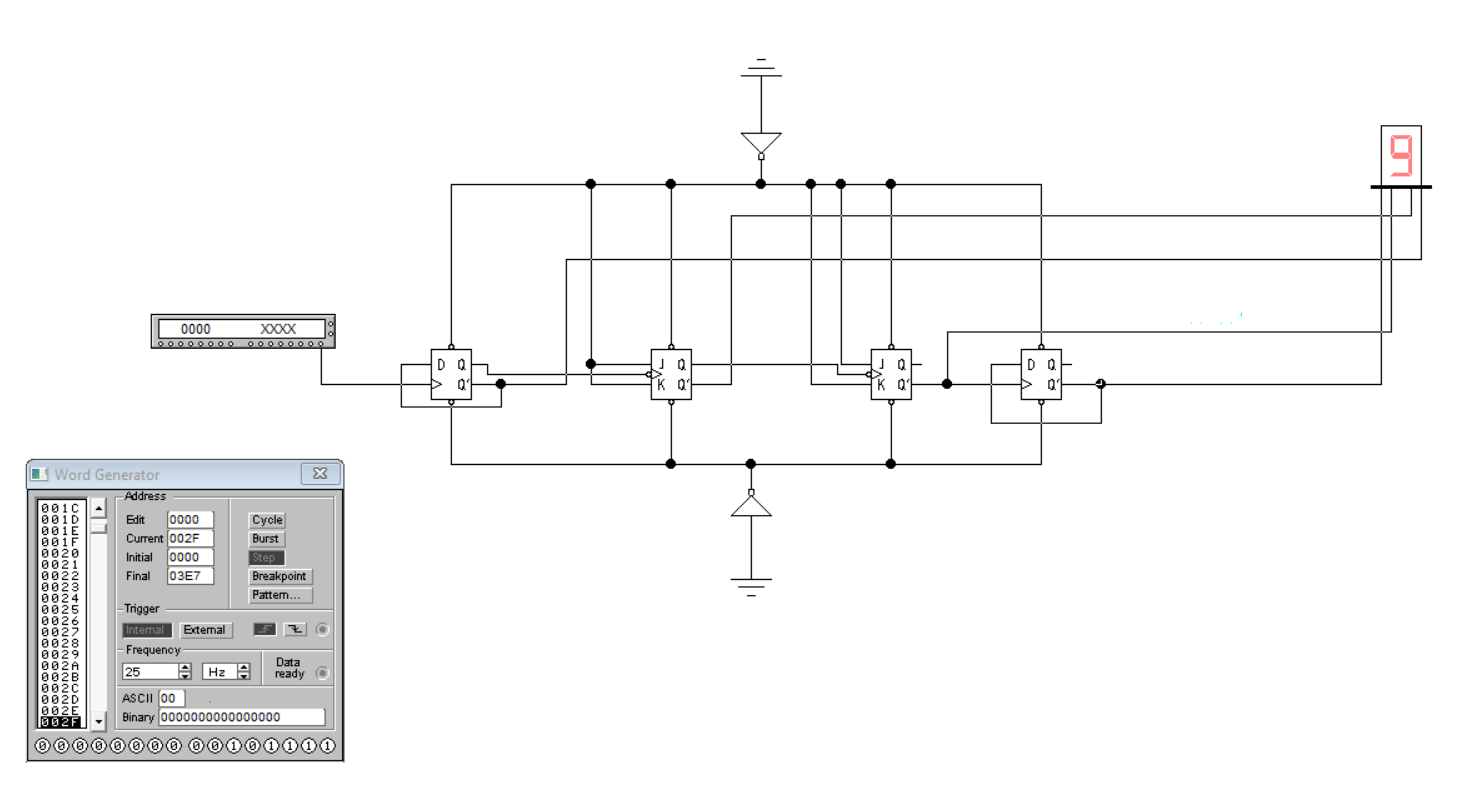
\includegraphics[width=\textwidth]{scheme_sub.png}
    \caption{Блок-схема вычитающего счетчика.}
    \label{fig:scheme_sub}
\end{figure}

Данный счетчик работает корректно.

\subsection*{Выводы}
В данной работе были построены счетчики (суммирующий и вычитающий) для двоично-десятичного кода. \\
По выданному варианту, необходимо было построить счетчики на двух типах триггеров $D$ и $JK$. Также для суммирующего необходимо было организовать обратную связь для сброса значений после числа $8$. \\
Используя теорию, были построены блок-схемы для счетчиков и затем проверена их работа по выходу индикатора. Результаты отображаемые на индикаторе полностью совпали с тем, для чего строилась схема, а значит работы была проделана верно.

\end{document}